\section{RationalGRL Methodology and Metamodel}
\label{sect:overview}

In this section we present a high-level overview of the RationalGRL framework. In the first subsection we present a methodology, specifying how practitioners can use RationalGRL to create goal models with traceability links to underlying arguments. In the second subsection we link the new argumentation elements and relations to the existing elements and relations of GRL in a metamodel. This metamodel serves as the specification for an implementation. In Section~\ref{sect:tool} we briefly discuss our prototype implementation based on this metamodel.

\subsection{RationalGRL Methodology} \todo{Sepideh}{Marc}{Review this section and make sure it is correct}

As mentioned in Section~\ref{sect:introduction}, the RationalGRL framework has been extended with concepts from practical reasoning argument scheme (PRAS) to help integrating goal models with the detailed discussions and arguments the stakeholders pose during the analysis phase. That is, the RationalGRL framework includes two main parts: Argumentation model and GRL model. 

To develop the argumentation model, we need to analyze critical questions, argument schemes and the stakeholder's discussions. For the GRL part of the framework, we first need to create the "initial" GRL models by analyzing the non-functional requirements in the requirements specification document and by refining the high-level goals into operationalized tasks. These two parts, GRL and argumentation models are developed iteratively and each side can impact the other side so that the models can be refined or new critical questions and argument schemes can be instantiated. For example, answering a critical question \emph{Is the task \texttt{A} possible?}, instantiated from the argumentation model, can result in removing or adding a task in the GRL model. Similarly,  if, for example, we add a new intentional element to the GRL model, it can lead to a new critical question relevant to this intentional element and its relationships with other intentional elements. Figure~\ref{fig:rationalgrl-framework} presents an overview of RationalGRL framework with its components and their relationships.  The GRL models  are shown  on the right-hand side of the framework while the argumentation models is on the left-hand side. The links between the two sides illustrates the impacts and relationships between two sides. 

\begin{figure}[ht]
\centering
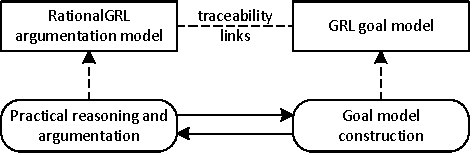
\includegraphics[scale=0.4]{img/framework}
\caption{The RationalGRL Framework}
\label{fig:rationalgrl-framework}
\end{figure}

We propose the following methodology (shown in Figure~\ref{fig:rationalgrl-methodology}) to develop an instance of the RationalGRL framework. Note that, here we assume that the initial GRL models have been created based on the requirements specification documents and the discussions of the stakeholders. The rest of the steps are as follows:

\begin{figure*}[ht]
\centering

\includegraphics[scale=0.4]{img/methodology}
\caption{The RationalGRL Methodology}
\label{fig:rationalgrl-methodology}
\end{figure*}

%TODO I need to reword up to the example.

\textbf{Instantiate Argument Schemes (AS)} -- After creating the initial GRL models, we In the first step, we instantiate one of the AS from the argumentation framework. In the section we develop 13 arguments schemes which we use in our analysis. An example of an argument scheme is "Goal \emph{G} contributes to softgoal \emph{S}". An instantiation of an argument scheme thus corresponds to an argument for or against part of a goal model.

\textbf{Answer Critical Questions (CQs)} -- Instantiated arguments can be attacked by counter-arguments. CQs are ways in which AS can be attacked. Each argument scheme includes one or more CQs. For example, for the argument scheme mentioned above, we have two CQs as: \emph{Does the goal contributes to the softgoal?} and \emph{Does the goal contributes to some other softgoals?}. Note that, the answer to CQ can also result into ``conflict'' situation which we do not consider here. Answering a CQ may result in an instantiation of a new AS. Thus, it is possible to go back and forth between this step and the previous one.

\textbf{Decide on IE and the Relationships} -- The answers to the CQs can result in one of the four cases which impact the arguments and corresponding GRL IE: \textsf{INTRO}, \textsf{DISABLE}, \textsf{REPLACE} or \textsf{ATTACK}.  \textsf{INTRO} means that the argument scheme of the CQ does not get attacked and instead it creates a new argument. \textsf{DISABLE} means that the IE or the relationship related to the AS needs to be disabled or removed from the models. \textsf{REPLACE} introduces a new argument and attack the original argument at the same time. It basically replace the original element of the AS with a new one.  \textsf{ATTACK} is a generic counterargument which attacks any argument with another argument when a new evidence occur.  

\textbf{Modify GRL Models} -- Based on the result of step three, the GRL models can be modified. In this case, either a new IE or a new relationships is introduced, an existing IE or relationship gets disabled (removed) from the model or finally an existing IE or relationships is replaced by a new one. This results in a new modified GRL. The new GRL model can then impact the argument schemes and instantiate another argument scheme.   

In the next section, we provide a short example to illustrate the relationship between argumentation framework and goal models. 

\subsubsection*{Example} \todo{Sepideh}{Marc}{Do we need an example here? I think no...this is from istar also, if we want it, we need to modify it}
\label{sect:methodology-example}

Our examples comes from a transcript containing discussions about the development of an information system, and they are created as part of two master theses on improving design reasoning~\cite{masterthesis1,masterthesis2}. We provide several more examples in Section~\ref{sect:examples}.

A group of stakeholders is developing a goal model for a traffic simulator example and they are modeling the goal \emph{simulate} of the system using the RationalGRL methodology. This proceeds in the following way:
\begin{itemize}
\item
First they start at step \emph{Modify GRL models} (Figure~\ref{fig:rationalgrl-methodology}), and add the IE \texttt{Simulate} to GRL model (Figure~\ref{fig:examples:decomposition}, GRL model, top IE).
\item Next, they switch to the argumentation part (step \emph{Instantiate arguments schemes}). They answer CQ \emph{Does Simulate AND-decompose into any tasks?} with \emph{Yes: namely tasks ``Dynamic simulation'' and ``Static simulation}.
\item As a result, two argument schemes are created, namely:
\begin{itemize}
\item Actor \emph{System} has task \emph{Dynamic simulation}
\item Actor \emph{System} has task \emph{Static simulation}
\end{itemize}
\item In the GRL model, this corresponds to the addition of two tasks, and an AND-decomposition from the goal \emph{Simulate} to these two tasks.
\item Next, the stakeholders test the validity of their goal model by answering more CQ. They answer two CQs:
\begin{itemize}
\item
CQ \emph{Is task ``Dynamic simulation'' relevant} is answered with ``No, it is not relevant since the problem specification explicitly states dynamic simulations are not required''. Thus, the corresponding GRL IE is disabled.
\item The decomposition is changed from AND to OR, since it turned out not both tasks can be implemented together.
\end{itemize}
\end{itemize}

The resulting RationalGRL model is shown in Figure~\ref{fig:examples:decomposition}, which can be found in Section~\ref{sect:examples}, where we will also explain the visualization of the examples in more detail.

\subsection{Metamodel}

\todo{Marc}{all}{This section is copy/pasted from RENext, we should revise the metamodel and the text.}

Figure~\ref{fig:metamodel} depicts the metamodel linking the main elements of our argumentation extension to the main GRL elements. The part below the dashed horizontal line depicts GRL elements. A \textsf{GRL Diagram} (bottom) contains zero or more \textsf{IntentionalElements}, either a \textsf{Goal}, a \textsf{Softgoal}, a \textsf{Task}, or a \textsf{Belief}. An \textsf{ElementLink} is either a \textsf{Contribution}, a \textsf{Decomposition}, or a \textsf{Dependency} and contains an \textsf{IntentionalElements} as source and as target.

The part above the horizontal dashed line depicts the concepts we introduced in the previous section. The top-left element \textsf{Argument} (see Section~\ref{sect:arguments}) can attack other arguments (Section~\ref{sect:attacks}) and generalizes both a \textsf{Formula} and an \textsf{Inference}. That is, both these elements can be arguments. A formula has an \textsf{AcceptStatus} (Section~\ref{sect:extensions}). An \textsf{Inference} is from a set of \textsf{Arguments} as premise and a \textsf{Formula} as conclusion. The \textsf{InferenceType} is either strict or defeasible (Section~\ref{sect:aspic}). A \textsf{Formula} is either a \textsf{Modality} (modal formula), a \textsf{Proposition}, a \textsf{BinaryOperation}, or a \textsf{Negation} (negated proposition). The \textsf{Modality} can be either B (belief), G (goal), E (evidence), or A (action). A \textsf{BinaryOperation} is either a \textsf{Disjunction}, a \textsf{Conjunction}, or a \emph{contributes\_to} \textsf{Connective}~(\ref{sect:aspic}).

Finally, the red arrows depict how the two metamodels are integrated. The left arrow connects a GRL \textsf{IntentionalElement} with an argumentation \textsf{Modality}, where the mapping is denoted with red text. Thus, an intention element traces to an argument, which is always a modal formula. The right arrow connects the GRL \textsf{ElementLink} with the argumentation \textsf{Connective} (i.e. a \emph{contributes\_to} connective). Thus, an arrow between elements of a GRL model corresponds to \emph{contributes\_to} connectives in the argumentation framework.

\begin{figure}[h!]
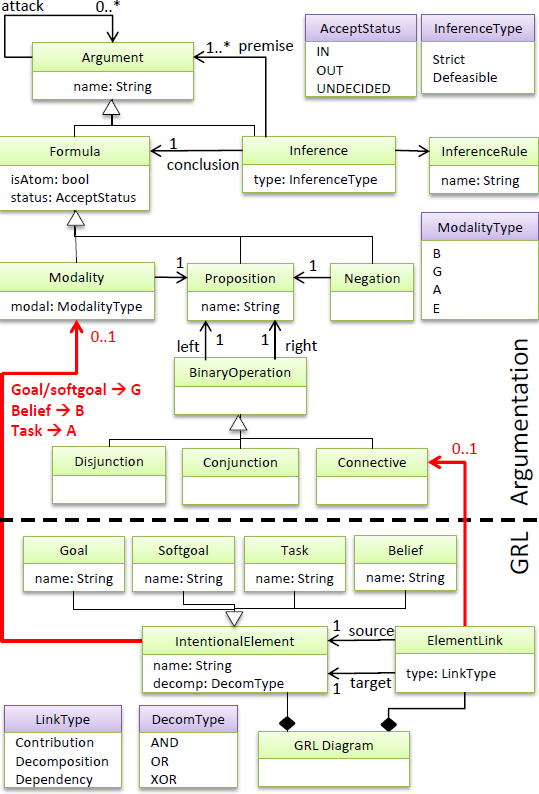
\includegraphics[scale=0.61]{img/metamodelimg}
\caption{The Metamodel \todo{Marc}{all}{This has to be revised.}}
\label{fig:metamodel}
\end{figure}